\section{线性规划的对偶}
\label{sec:lp-duality}

有人告诉我们，车间问题的最优解是$(2,2)$，最大利润是$10$。检查可行性只需代入约束，难的是确认没有更好的产量。怎样给出一份不依赖求解过程、能当场核对的最优性证据？答案来自第~\ref{chap:optimization}章用过的办法，把约束加起来，只是这次要系统地做。

\paragraph{给约束配权重}
把工时约束乘以$u_1\geq0$，原料约束乘以$u_2\geq0$，再相加。权重非负，不等号方向不变，得到
\[
 (u_1+2u_2)x_1+(u_1+u_2)x_2\leq4u_1+6u_2.
\]
如果左边的系数“盖得住”利润系数，也就是
\[
 u_1+2u_2\geq3,\qquad u_1+u_2\geq2,
\]
那么由$x_1,x_2\geq0$，任何可行产量的利润都不超过$4u_1+6u_2$。

不同的权重给出不同的上界。下面四组权重都满足上述条件：
\[
 \bm{u}=(2,1)\to14,\quad(3,0)\to12,\quad(0,2)\to12,\quad(1,1)\to10.
\]
最后一个上界$10$恰好等于$(2,2)$的利润，所以$(2,2)$最优。这一行计算不依赖任何算法，谁都可以复核。

权重可以读成资源的价格。设想有人想买下车间全部的工时和原料，出价$u_1,u_2$。车间只在卖资源不比自己生产亏时才肯卖，这就是上面的两个不等式。买方希望总价$4u_1+6u_2$尽量低，寻找最低总价就是寻找最紧的上界，于是有问题
\begin{equation}
 \min_{u_1,u_2}\ 4u_1+6u_2
 \quad\text{s.t.}\quad u_1+2u_2\geq3,\quad u_1+u_2\geq2,\quad u_1,u_2\geq0.
 \label{eq:lp-workshop-prices}
\end{equation}
图~\ref{fig:lp-dual-bounds}(a)是这个问题的可行域，最低总价$10$在$(1,1)$取得。图~\ref{fig:lp-dual-bounds}(b)把两边的数放在同一条数轴上：每个产量的利润都在每个价格的总价左边，两者在$10$处相遇。这正是“上下界夹逼”。买卖的故事只用来说明不等式的方向，并不表示真有这样一个市场，价格只是一组使不等式成立的数。

\begin{BookInlineFigure}
 \centering
 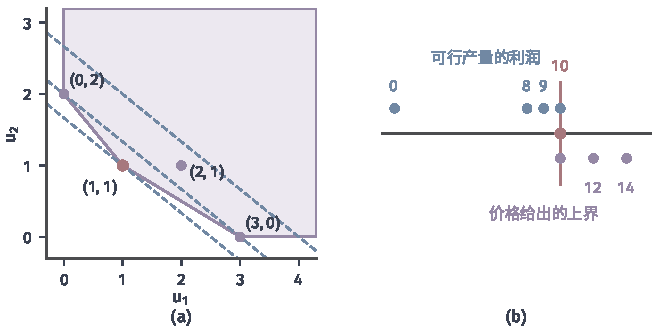
\includegraphics[width=112mm]{figures/05-optimization/01-linear-programming/matplotlib/lp-dual-bounds/figure.pdf}
 \caption{资源价格给出的上界。(a)~浅紫区域是满足式~\eqref{eq:lp-workshop-prices}约束的价格$(u_1,u_2)$，蓝色虚线是总价$10,12,16$的等值线，红点$(1,1)$是最低总价。(b)~数轴上方的蓝点是四个顶点的利润$0,8,9,10$，下方的紫点是四组价格的总价$10,12,14$，红线标出两侧在$10$处相遇。}
 \label{fig:lp-dual-bounds}
\end{BookInlineFigure}

\paragraph{标准型的对偶问题}
对标准型~\eqref{eq:lp-standard}做同样的事。约束是等式，乘以任意实数都不改变等号，所以第$i$个等式的权重$y_i$没有符号限制。把等式按权重相加，得到
\[
 \bm{y}^\top\bm{A}\bm{x}=\bm{b}^\top\bm{y}.
\]
我们想用左边给目标$\bm{c}^\top\bm{x}$找下界。记两者系数的差为$\bm{s}=\bm{c}-\bm{A}^\top\bm{y}$，则
\[
 \bm{c}^\top\bm{x}=\bm{y}^\top\bm{A}\bm{x}+\bm{s}^\top\bm{x}=\bm{b}^\top\bm{y}+\bm{s}^\top\bm{x}.
\]
只要$\bm{s}\geq\bm{0}$，由$\bm{x}\geq\bm{0}$知$\bm{s}^\top\bm{x}\geq0$，于是$\bm{b}^\top\bm{y}$就是下界。求最好的下界，就得到下面的问题。

\begin{definition}[线性规划的对偶问题]
 \label{def:lp-dual}
 标准型~\eqref{eq:lp-standard}的\term{对偶问题}（dual problem）是
 \begin{equation}
  \max_{\bm{y}\in\mathbb{R}^m,\ \bm{s}\in\mathbb{R}^n}\ \bm{b}^\top\bm{y}
  \quad\text{s.t.}\quad\bm{A}^\top\bm{y}+\bm{s}=\bm{c},\quad\bm{s}\geq\bm{0},
  \label{eq:lp-dual}
 \end{equation}
 其中$\bm{y}$没有符号限制，$\bm{s}$称为\term{对偶松弛}（dual slack），最优值记为$d^\star$。相对地，式~\eqref{eq:lp-standard}称为\term{原始问题}（primal problem）。
\end{definition}

对偶的每个$s_j$对应原始的一个变量$x_j$，对偶的每个$y_i$对应原始的一个等式。把车间问题的标准型~\eqref{eq:lp-workshop-standard}代入，得到
\[
 s_1=-3-y_1-2y_2,\quad s_2=-2-y_1-y_2,\quad s_3=-y_1,\quad s_4=-y_2.
\]
$s_3,s_4\geq0$说的是$y_1,y_2\leq0$，这个符号来自松弛变量的列。令$\bm{u}=-\bm{y}$，$s_1,s_2\geq0$就是式~\eqref{eq:lp-workshop-prices}的两个不等式，对偶目标$4y_1+6y_2$变为$-(4u_1+6u_2)$。两种写法只差一个符号，因为这里把最大利润改成了最小化相反数。

\begin{theorem}[弱对偶]
 \label{thm:lp-weak-duality}
 若$\bm{x}$对原始问题可行，$(\bm{y},\bm{s})$对对偶问题可行，则
 \begin{equation}
  \bm{c}^\top\bm{x}-\bm{b}^\top\bm{y}=\bm{x}^\top\bm{s}\geq0.
  \label{eq:lp-weak-duality}
 \end{equation}
 特别地$d^\star\leq p^\star$；若$\bm{x}^\top\bm{s}=0$，则$\bm{x}$和$(\bm{y},\bm{s})$分别是两个问题的最优解。
\end{theorem}

\begin{proof}
 把$\bm{c}=\bm{A}^\top\bm{y}+\bm{s}$代入，再用$\bm{A}\bm{x}=\bm{b}$，得到
 \[
  \bm{c}^\top\bm{x}=\bm{y}^\top\bm{A}\bm{x}+\bm{s}^\top\bm{x}=\bm{b}^\top\bm{y}+\bm{x}^\top\bm{s}.
 \]
 两个向量都非负，所以$\bm{x}^\top\bm{s}\geq0$。

 若$\bm{x}^\top\bm{s}=0$，则$\bm{c}^\top\bm{x}=\bm{b}^\top\bm{y}$。任何其他原始可行点的目标值都不小于$\bm{b}^\top\bm{y}$，任何其他对偶可行点的目标值都不大于$\bm{c}^\top\bm{x}$，所以两者都最优。
\end{proof}

这个结论称为\term{弱对偶}（weak duality）。差$\bm{c}^\top\bm{x}-\bm{b}^\top\bm{y}$称为这对可行点的\term{对偶间隙}（duality gap）。它同时控制了两边：$\bm{c}^\top\bm{x}-p^\star$不超过间隙，$d^\star-\bm{b}^\top\bm{y}$也不超过间隙。

条件$\bm{s}\geq\bm{0}$不是形式要求。取价格$\bm{u}=(1/2,1)$，它满足$u_1+u_2\geq2$，却违反$u_1+2u_2\geq3$，因为左边是$5/2$。它算出的“上界”是$4u_1+6u_2=8$，比真实的最大利润$10$还小。对偶可行性没有检查，这个数就什么也不说明。

\paragraph{符号规则}
其他形式的原始问题对应什么样的对偶？不必记表，每次回到“加权相加后不等号方向要对”即可。表~\ref{tab:lp-sign-rules}是最小化问题的结果。例如$\bm{g}^\top\bm{x}\geq h$要用来给目标找下界，权重必须非负；$x_j$可正可负时，$s_jx_j$要始终非负，只能$s_j=0$。

\begin{BookInlineTable}
 \centering
 \begin{tabular}{ll}
  \toprule
  原始（最小化） & 对偶（最大化） \\
  \midrule
  等式约束 & 权重$y_i$无符号限制 \\
  $\geq$约束 & $y_i\geq0$ \\
  $\leq$约束 & $y_i\leq0$ \\
  $x_j\geq0$ & $s_j\geq0$ \\
  $x_j$自由 & $s_j=0$ \\
  $x_j\leq0$ & $s_j\leq0$ \\
  \bottomrule
 \end{tabular}
 \caption{最小化问题的对偶符号规则，其中$s_j=c_j-\bm{a}_j^\top\bm{y}$。}
 \label{tab:lp-sign-rules}
\end{BookInlineTable}

对偶的对偶回到原问题。把式~\eqref{eq:lp-dual}中的$\bm{y}$写成$\bm{y}^{+}-\bm{y}^{-}$，并把目标取相反数，它成为变量$\bm{y}^{+},\bm{y}^{-},\bm{s}$上的标准型：
\[
 \min\ -\bm{b}^\top\bm{y}^{+}+\bm{b}^\top\bm{y}^{-}
 \quad\text{s.t.}\quad
 \bm{A}^\top\bm{y}^{+}-\bm{A}^\top\bm{y}^{-}+\bm{s}=\bm{c}.
\]
按定义写出它的对偶，权重记为$\bm{z}$，三组列分别给出三组不等式：
\[
 \bm{A}\bm{z}\leq-\bm{b},\qquad-\bm{A}\bm{z}\leq\bm{b},\qquad\bm{z}\leq\bm{0}.
\]
前两组合起来是$\bm{A}\bm{z}=-\bm{b}$。令$\bm{x}=-\bm{z}$，这个对偶就是在$\bm{A}\bm{x}=\bm{b}$，$\bm{x}\geq\bm{0}$上最大化$-\bm{c}^\top\bm{x}$，也就是原来的标准型。两个问题的地位因此是对称的，表~\ref{tab:lp-primal-dual}用车间问题对照了它们的成分。

\begin{BookInlineTable}
 \centering
 \begin{tabular}{lll}
  \toprule
  & 原始：决定产量 & 对偶：决定价格 \\
  \midrule
  变量 & $x_j$，产品$j$的产量 & $u_i$，资源$i$的单价 \\
  约束 & 每种资源够用 & 每种产品的资源价值不低于利润 \\
  目标 & 最大化利润 & 最小化资源总价 \\
  相互给出 & 最大利润的下界 & 最大利润的上界 \\
  \bottomrule
 \end{tabular}
 \caption{车间问题的原始问题与对偶问题。原始的一条约束对应对偶的一个变量，原始的一个变量对应对偶的一条约束。}
 \label{tab:lp-primal-dual}
\end{BookInlineTable}

\paragraph{Farkas引理}
弱对偶只说明下界不超过最优值，下界能否恰好等于最优值？这要靠一个判定等式组可解性的定理。先看几何。$\{\bm{A}\bm{x}:\bm{x}\geq\bm{0}\}$是$\bm{A}$的各列按非负系数组合得到的锥，记作$\bm{K}$，等式组$\bm{A}\bm{x}=\bm{b}$，$\bm{x}\geq\bm{0}$有解就是$\bm{b}\in\bm{K}$。

如果$\bm{b}$在锥外，直觉告诉我们，应该有一个过原点的超平面把整个锥和$\bm{b}$隔在两侧。这个超平面的法向量$\bm{z}$就是不可解的证据。

\begin{theorem}[Farkas引理]
 \label{thm:lp-farkas}
 给定$\bm{A}\in\mathbb{R}^{m\times n}$和$\bm{b}\in\mathbb{R}^m$，下面两个系统恰有一个有解：
 \begin{align}
  &\bm{A}\bm{x}=\bm{b},\quad\bm{x}\geq\bm{0}; \label{eq:lp-farkas-primal}\\
  &\bm{A}^\top\bm{z}\geq\bm{0},\quad\bm{b}^\top\bm{z}<0. \label{eq:lp-farkas-dual}
 \end{align}
\end{theorem}

\begin{proof}
 两个系统不能同时有解，否则
 \[
  0>\bm{b}^\top\bm{z}=\bm{x}^\top\bm{A}^\top\bm{z}\geq0.
 \]

 现在设式~\eqref{eq:lp-farkas-primal}无解，即$\bm{b}\notin\bm{K}$，要构造$\bm{z}$。先证$\bm{K}$是闭集。任取$\bm{v}\in\bm{K}$，在$\bm{v}=\bm{A}\bm{x}$（$\bm{x}\geq\bm{0}$）的写法中取正分量最少的一种。若正分量对应的列线性相关，可以像引理~\ref{lem:lp-push}那样沿零空间方向移动，再消去一个正分量，矛盾。所以这些列线性无关，$\bm{K}$是有限多个集合$\bm{K}_J$的并，每个$\bm{K}_J$由一组线性无关的列$\bm{A}_J$按非负系数组合而成。

 设$\bm{A}_J\bm{x}^{(k)}\to\bm{v}$，$\bm{x}^{(k)}\geq\bm{0}$。$\bm{A}_J$列满秩，所以
 \[
  \bm{x}^{(k)}=(\bm{A}_J^\top\bm{A}_J)^{-1}\bm{A}_J^\top\bm{A}_J\bm{x}^{(k)}
 \]
 收敛，极限非负，于是$\bm{v}\in\bm{K}_J$。有限个闭集的并是闭集，$\bm{K}$闭。

 再取$\bm{K}$中离$\bm{b}$最近的点。任取$\bm{v}_0\in\bm{K}$，$\bm{K}$与以$\bm{b}$为中心、半径$\lVert\bm{v}_0-\bm{b}\rVert_2$的闭球之交是非空紧集，连续函数$\lVert\bm{v}-\bm{b}\rVert_2^2$在其上取得最小值，这个最小点$\widehat{\bm{v}}$就是$\bm{K}$上的最小点。令
 \[
  \bm{z}=\widehat{\bm{v}}-\bm{b}\neq\bm{0}.
 \]

 $\bm{K}$是锥，所以对每个$t\geq0$，$t\widehat{\bm{v}}\in\bm{K}$。函数$\phi(t)=\lVert t\widehat{\bm{v}}-\bm{b}\rVert_2^2$在$t=1$取最小，导数$\phi'(1)$为零，也就是$2\widehat{\bm{v}}^\top\bm{z}=0$，所以（$\widehat{\bm{v}}=\bm{0}$时等式自然成立）
 \[
  \widehat{\bm{v}}^\top\bm{z}=0.
 \]
 对每一列$\bm{a}_j$和$t\geq0$，点$\widehat{\bm{v}}+t\bm{a}_j$也在$\bm{K}$中，所以它到$\bm{b}$的距离平方在$t=0$处的右导数$2\bm{a}_j^\top\bm{z}$非负，得到
 \[
  \bm{a}_j^\top\bm{z}\geq0.
 \]
 这就是$\bm{A}^\top\bm{z}\geq\bm{0}$。最后，由$\bm{b}=\widehat{\bm{v}}-\bm{z}$和$\widehat{\bm{v}}^\top\bm{z}=0$，
 \[
  \bm{b}^\top\bm{z}=\widehat{\bm{v}}^\top\bm{z}-\lVert\bm{z}\rVert_2^2=-\lVert\bm{z}\rVert_2^2<0.
 \]
\end{proof}

满足式~\eqref{eq:lp-farkas-dual}的$\bm{z}$是不可行的证书。核对它只需一次矩阵乘法：若有可行的$\bm{x}$，$\bm{b}^\top\bm{z}=\bm{x}^\top\bm{A}^\top\bm{z}$是非负数的乘积之和，不可能为负。

用车间矩阵的前两列看两种情形，这两列是
\[
 \bm{a}_1=(1,2)^\top,\qquad\bm{a}_2=(1,1)^\top.
\]
右端为$\bm{b}=(4,6)^\top$时，$\bm{x}=(2,2)^\top$是解，如图~\ref{fig:lp-farkas-cone}(a)。右端换成$\bm{b}'=(1,0)^\top$时，解方程组得$x_1=-1$，$x_2=2$，没有非负解。按证明构造：锥$\bm{K}$上离$\bm{b}'$最近的点在$\bm{a}_2$这条边上，
\[
 \widehat{\bm{v}}=\Bigl(\frac12,\frac12\Bigr)^\top,\qquad\bm{z}=\widehat{\bm{v}}-\bm{b}'=\Bigl(-\frac12,\frac12\Bigr)^\top.
\]
逐项核对：
\[
 \bm{a}_1^\top\bm{z}=\frac12,\qquad\bm{a}_2^\top\bm{z}=0,\qquad(\bm{b}')^\top\bm{z}=-\frac12.
\]
这组权重的含义也很直接：第二个等式减第一个等式，得到$x_1=-1$，与$x_1\geq0$矛盾。

\begin{BookInlineFigure}
 \centering
 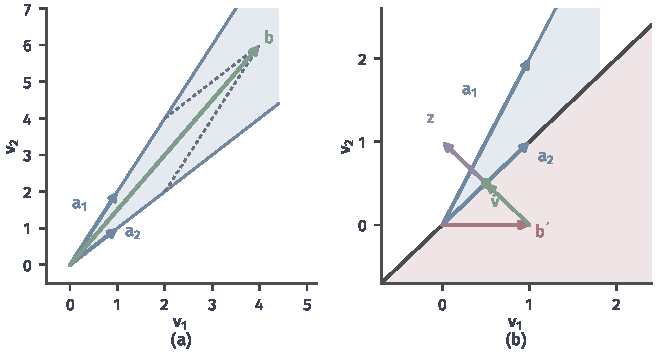
\includegraphics[width=112mm]{figures/05-optimization/01-linear-programming/matplotlib/lp-farkas-cone/figure.pdf}
 \caption{Farkas引理的几何。蓝色箭头是两列$\bm{a}_1,\bm{a}_2$，浅蓝区域是它们张成的锥。(a)~$\bm{b}=(4,6)^\top$在锥内，灰色虚线是$\bm{b}=2\bm{a}_1+2\bm{a}_2$的分解。(b)~$\bm{b}'=(1,0)^\top$在锥外，绿点$\widehat{\bm{v}}$是锥上最近的点，紫色箭头$\bm{z}=\widehat{\bm{v}}-\bm{b}'$是分离超平面（深灰线）的法向量；浅红半平面是$\bm{z}^\top\bm{v}<0$的一侧，$\bm{b}'$在其中，整个锥在另一侧。}
 \label{fig:lp-farkas-cone}
\end{BookInlineFigure}

\paragraph{强对偶}
现在回答开头的问题：只要原始问题可行且最优值有限，最好的下界就等于最优值，这个结论称为\term{强对偶}（strong duality）。

\begin{theorem}[线性规划强对偶]
 \label{thm:lp-strong-duality}
 若标准型~\eqref{eq:lp-standard}可行且最优值$p^\star$有限，则对偶问题~\eqref{eq:lp-dual}有最优解，并且
 \begin{equation}
  d^\star=p^\star.
  \label{eq:lp-strong-duality}
 \end{equation}
\end{theorem}

\begin{proof}
 只需找到$(\bm{y},\bm{s})$对偶可行，且$\bm{b}^\top\bm{y}\geq p^\star$，弱对偶就会迫使等号成立。把要求写成带非负变量的等式组，引入$r\geq0$，令$\bm{y}=\bm{y}^{+}-\bm{y}^{-}$：
 \[
  \bm{A}^\top\bm{y}^{+}-\bm{A}^\top\bm{y}^{-}+\bm{s}=\bm{c},\qquad
  \bm{b}^\top\bm{y}^{+}-\bm{b}^\top\bm{y}^{-}-r=p^\star.
 \]

 假设这个系统没有非负解。由Farkas引理，存在$\bm{z}\in\mathbb{R}^n$和$\sigma\in\mathbb{R}$，对系数矩阵的四组列分别满足
 \[
  \bm{A}\bm{z}+\sigma\bm{b}\geq\bm{0},\quad
  -\bm{A}\bm{z}-\sigma\bm{b}\geq\bm{0},\quad
  \bm{z}\geq\bm{0},\quad
  -\sigma\geq0,
 \]
 并且右端的内积为负，即$\bm{c}^\top\bm{z}+\sigma p^\star<0$。记$\tau=-\sigma\geq0$，前两式合起来得到
 \[
  \bm{A}\bm{z}=\tau\bm{b},\qquad\bm{z}\geq\bm{0},\qquad\bm{c}^\top\bm{z}<\tau p^\star.
 \]

 若$\tau>0$，则$\bm{z}/\tau$是原始可行点，目标值小于$p^\star$，矛盾。若$\tau=0$，则$\bm{A}\bm{z}=\bm{0}$，$\bm{z}\geq\bm{0}$，$\bm{c}^\top\bm{z}<0$。任取可行点$\widehat{\bm{x}}$，$\widehat{\bm{x}}+t\bm{z}$对一切$t\geq0$可行，目标趋于$-\infty$，与$p^\star$有限矛盾。

 所以系统有解，得到对偶可行的$(\bm{y},\bm{s})$和$\bm{b}^\top\bm{y}=p^\star+r\geq p^\star$。由弱对偶，$\bm{b}^\top\bm{y}\leq p^\star$，因此$\bm{b}^\top\bm{y}=p^\star$，这个$(\bm{y},\bm{s})$是对偶最优解。
\end{proof}

证明里两种情形各用了一个条件：$\tau>0$时用到$p^\star$是下确界，$\tau=0$时用到问题可行且有下界。线性规划的强对偶不需要其他条件。一般的凸问题则不然，第~\ref{chap:duality}章会在Lagrange函数的框架下说明，零间隙还需要额外的假设。

\paragraph{互补松弛与零间隙证书}
强对偶告诉我们证书一定存在，弱对偶告诉我们怎样核对它。把两者合起来，就是线性规划的最优性判别。

\begin{theorem}[零间隙证书与互补松弛]
 \label{thm:lp-optimality-certificate}
 设标准型的$\bm{x}$和$(\bm{y},\bm{s})$满足
 \begin{equation}
  \bm{A}\bm{x}=\bm{b},\quad\bm{x}\geq\bm{0},\qquad
  \bm{A}^\top\bm{y}+\bm{s}=\bm{c},\quad\bm{s}\geq\bm{0}.
  \label{eq:lp-pd-feasible}
 \end{equation}
 则下面三条等价：$\bm{x}$和$(\bm{y},\bm{s})$分别是原始、对偶最优解；$\bm{c}^\top\bm{x}=\bm{b}^\top\bm{y}$；对每个$j$，
 \begin{equation}
  x_js_j=0.
  \label{eq:lp-complementary}
 \end{equation}
\end{theorem}

\begin{proof}
 由式~\eqref{eq:lp-weak-duality}，第二条等价于$\bm{x}^\top\bm{s}=0$。$\bm{x}^\top\bm{s}$是非负数$x_js_j$之和，为零当且仅当每一项为零，这就是第三条。第二条推出第一条是弱对偶的结论。反过来若两者都最优，由强对偶知两个最优值相等，得到第二条。
\end{proof}

式~\eqref{eq:lp-complementary}称为\term{互补松弛}（complementary slackness）。它说的是，每对$(x_j,s_j)$中至少有一个为零。用价格的语言：正在生产的产品没有多余的利润，有多余的资源价格为零。第~\ref{chap:lp-interior-point}章的算法正是围绕这组方程组织的。

有了最优解的猜测，互补松弛还能反过来求出价格。车间问题中$\bm{x}^\star=(2,2,0,0)^\top$，$x_1,x_2>0$要求$s_1=s_2=0$，也就是
\[
 y_1+2y_2=-3,\qquad y_1+y_2=-2.
\]
解得$\bm{y}=(-1,-1)^\top$，再算出其余的对偶松弛：
\[
 s_3=-y_1=1,\qquad s_4=-y_2=1.
\]
$\bm{s}=(0,0,1,1)^\top\geq\bm{0}$，对偶可行，并且$\bm{b}^\top\bm{y}=-10=\bm{c}^\top\bm{x}^\star$。这一对点就是最优性的完整证书。

不是最优的顶点通不过同样的检查。取$(3,0)$，即$\bm{x}=(3,0,1,0)^\top$。$x_1,x_3>0$要求$s_1=s_3=0$，于是
\[
 y_1=0,\qquad y_2=-\frac32,\qquad s_2=-2-y_1-y_2=-\frac12<0.
\]
满足互补松弛的$\bm{y}$只有这一个，它不对偶可行，所以$(3,0)$不是最优解。

这个判别有直接的几何含义。回到平面上，顶点处的活动约束有各自的外法向量。互补松弛说的是，利润向量$\bm{p}$是活动约束法向量的非负组合。图~\ref{fig:lp-normal-cone}在两个顶点上比较：$(2,2)$处$\bm{p}=1\cdot\bm{n}_1+1\cdot\bm{n}_2$，系数正是价格$\bm{u}=(1,1)$；$(3,0)$处活动约束的法向量是$\bm{n}_2=(2,1)$和$\bm{n}_3=(0,-1)$，分解
\[
 \begin{bmatrix}3\\2\end{bmatrix}=\frac32\begin{bmatrix}2\\1\end{bmatrix}-\frac12\begin{bmatrix}0\\-1\end{bmatrix}
\]
含负系数，$\bm{p}$在锥外，负系数$-1/2$正是上面算出的$s_2$。

\begin{BookInlineFigure}
 \centering
 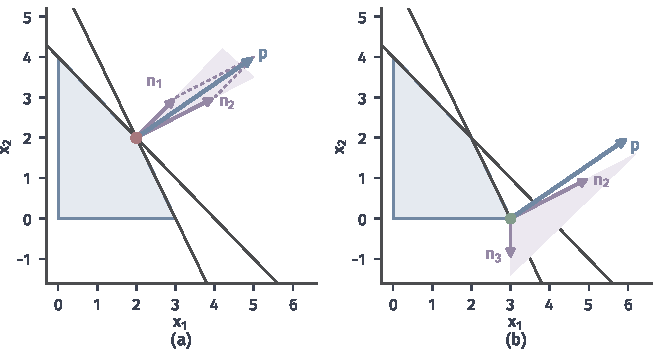
\includegraphics[width=112mm]{figures/05-optimization/01-linear-programming/matplotlib/lp-normal-cone/figure.pdf}
 \caption{互补松弛的几何。紫色箭头是顶点处活动约束的外法向量，浅紫区域是它们张成的锥，蓝色箭头是利润向量$\mathbf{p}=(3,2)$。(a)~$(2,2)$处，$\mathbf{p}$在锥内，是两个法向量的正组合（紫色虚线），该顶点最优。(b)~$(3,0)$处，$\mathbf{p}$在锥外，该顶点不是最优解。}
 \label{fig:lp-normal-cone}
\end{BookInlineFigure}

价格还有边际价值的含义。把工时从$4$增加到$5$，新的最优产量是$(1,4)$，利润$11$，恰好增加$u_1=1$。这种关系只在一定范围内成立，第~\ref{chap:simplex-method}章固定最优基时会算出这个范围。

\paragraph{三种结局的证书}
线性规划只有三种结局，每种都有可以独立核对的证据。有最优解时，证书是满足式~\eqref{eq:lp-pd-feasible}和式~\eqref{eq:lp-complementary}的一对点。不可行时，证书是满足式~\eqref{eq:lp-farkas-dual}的$\bm{z}$。无下界时，证书是一个可行点加上满足下式的方向：
\begin{equation}
 \bm{A}\bm{d}=\bm{0},\qquad\bm{d}\geq\bm{0},\qquad\bm{c}^\top\bm{d}<0.
 \label{eq:lp-unbounded-certificate}
\end{equation}

两个问题的结局也互相牵制。原始无下界时，对偶不可能有可行点，否则弱对偶会给出有限下界，所以对偶不可行。由对称性，对偶无上界时原始不可行。两者都不可行的情形确实存在，例如
\[
 \min\ -x_1-x_2\quad\text{s.t.}\quad x_1-x_2=1,\quad-x_1+x_2=1,\quad\bm{x}\geq\bm{0}.
\]
两个等式相加得到$0=2$，原始不可行；对偶约束$y_1-y_2\leq-1$和$-y_1+y_2\leq-1$相加得到$0\leq-2$，对偶也不可行。

这个例子中方向$\bm{d}=(1,1)^\top$满足式~\eqref{eq:lp-unbounded-certificate}，但没有可行的起点，它什么也说明不了。所以报告无下界时，可行点和方向缺一不可。表~\ref{tab:lp-outcomes}列出全部可能的组合。

\begin{BookInlineTable}
 \centering
 \begin{tabular}{llll}
  \toprule
  原始＼对偶 & 有最优解 & 无上界 & 不可行 \\
  \midrule
  有最优解 & 可能，且$p^\star=d^\star$ & 不可能 & 不可能 \\
  无下界 & 不可能 & 不可能 & 可能 \\
  不可行 & 不可能 & 可能 & 可能 \\
  \bottomrule
 \end{tabular}
 \caption{原始问题与对偶问题结局的组合。两个“有最优解”以外的“不可能”分别由强对偶、弱对偶和对称性得到。}
 \label{tab:lp-outcomes}
\end{BookInlineTable}

\paragraph{图中的流问题}
第~\ref{sec:lp-formulation}节的网络流实例能让对偶问题有具体的含义。关联矩阵~\eqref{eq:lp-network-data}的列是$\bm{a}_{i,j}=\bm{e}_i-\bm{e}_j$，所以$\bm{a}_{i,j}^\top\bm{y}=y_i-y_j$，对偶约束是逐弧的不等式，这里$\bm{e}_i$是第$i$个单位向量：
\begin{equation}
 s_{i,j}=c_{i,j}-(y_i-y_j)\geq0.
 \label{eq:lp-network-dual}
\end{equation}
$y_i$是节点上的数，可以读成“从节点$i$把一单位货物送到终点的费用估计”，这种量通常称为节点势。式~\eqref{eq:lp-network-dual}要求沿弧走一步，费用估计的下降不能超过这条弧的费用。对偶目标$\bm{b}^\top\bm{y}=y_1-y_4$是起点和终点的势差。

矩阵的四行线性相关，这时$\bm{y}$可以整体加一个常数而不影响任何$y_i-y_j$，所以取$y_4=0$，这相当于删去第四行。令最短路$1\to2\to3\to4$上的三条弧都取等号，得到
\[
 y_3=2,\qquad y_2=y_3+1=3,\qquad y_1=y_2+2=5.
\]
其余两条弧的对偶松弛为
\[
 s_{1,3}=5-(5-2)=2,\qquad s_{2,4}=6-(3-0)=3.
\]

路径$1\to2\to3\to4$的流量为$1$，总费用$2+1+2=5$，而$\bm{b}^\top\bm{y}=5-0=5$，两者相等。图~\ref{fig:lp-network-dual}显示了这份证书，互补松弛说的是：只有$s_{i,j}=0$的弧上才允许有流量。

\begin{BookInlineFigure}
 \centering
 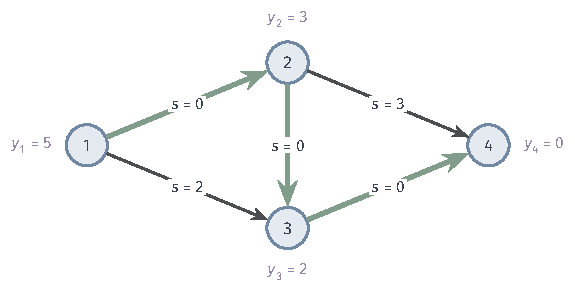
\includegraphics[width=97mm]{figures/05-optimization/01-linear-programming/tikz/lp-network-dual/figure.pdf}
 \caption{图~\ref{fig:lp-network-instance}实例的对偶证书。节点旁的紫色数字是节点势$y_i$，弧旁是对偶松弛$s_{i,j}$。绿色粗线是流量为$1$的最短路，这些弧上$s_{i,j}=0$，其余两条弧无流量。}
 \label{fig:lp-network-dual}
\end{BookInlineFigure}

这份证书正是图算法中逐弧检查的最优性条件。最短路的逐弧不等式和最小费用流的节点势都是对偶可行性，可参考\BookChapterRef{chap:shortest-paths}{卷三第3章“最短路”}；最大流最小割定理也是这种配对关系的特例，割给出流量的上界，可参考\BookChapterRef{chap:max-flow-min-cut}{卷三第5章“最大流与最小割”}。一般凸问题的对偶由第~\ref{chap:duality}章用Lagrange函数统一处理，线性规划是其中条件最宽松的情形。
